\chapter{Anwenderdokumentation}
\section{Produktzweck}
Eines der wohl wichtigsten Werkzeugen nicht nur im Studium, sondern 
auch in Berufen speziell in der Forschung und Entwicklung, sind B"ucher. 
Allerdings ist der Umfang von Fachliteratur nicht unbedingt klein und 
"uberschaubar. Au"serdem kann ein Fehlkauf sehr schnell ins Geld gehen, 
bei B"ucherpreisen von 50 EUR und mehr.\\
Wie w"are es also mit einem Werkzeug um Informationen "uber diese 
Werkzeuge "ubersichtlich bereit zu stellen.\\
Informationen wie Titel, Autor und ISBN werden von 
Migliedern verfasst und in einer Datenbank abgelegt. Aber 
damit nicht genug, es ist jedem Mitglied auch m"oglich Kommentare zu 
verfassen, z. B. wie ihm das Buch gefallen hat oder ob es bei Recherchen "uber gewisse Themen
hilfreich war oder nicht.\\
Um einen universellen Zugriff auf die Datenbest"ande der Literaturverwaltung zu gew"ahrleisten, 
erfolgt der Zugriff "uber dynamisch erzeugte HTML-Seiten, die einfach 
mit jedem Web-Browser "uber die Web-Adresse aufgerufen werden k"onnen.\\
Ein weiterer Vorteil, den dynamisch erzeugte HTML-Seiten bieten ist die freie Plattformwahl durch den Nutzer.

\section{Basismaschine und Ressourcenanforderungen}
Die Literaturverwaltung wird von einem Administrator auf einem Web-Server installiert und konfiguriert. Dies erm"oglicht jedem Nutzer einen ortsunab"angigen Zugriff auf die Datenbest"ande.\\
Es wird lediglich ein Web-Browser wie z. B. Firefox, Opera oder der Internet Explorer ben"otigt.\\
Die Anforderungen an die Hardware richten sich nach den Anforderungen des benutzten Web-Browsers.

\section{Nutzerklassen}
Es gibt drei Nutzerklassen:
\begin{enumerate}
\item Nutzer:\\
Nutzer ist jeder, der sich "uber einen Web-Browser auf die Seite begibt um Informationen abzurufen.\\
Der Nutzer besitzt keinerlei M"oglichkeiten Datenbest"ande anzulegen, zu ver"andern oder zu l"oschen. Er besitzt lediglich Lesezugriff auf die Literaturinformationen und Kommentare. \\

\item Mitglied:\\
Das Mitglied ist ein registrierte Nutzer, der sich durch sein Anmelden "uber die grafische Oberfl"ache mit einem LogIn-Namen und einem Passwort als solcher authentifiziert.\\
Als Mitglied darf man zus"atzlich zu den Rechten eines Nutzers neue Literatur anlegen oder bereits bestehende Titel bearbeiten und l"oschen.\\
Desweiteren besitzt jedes Mitglied das Recht, Kommentare zu verfassen sowie eigens erstellte Kommentare zu bearbeiten und zu l"oschen.\\
Was die Mitgliedsdaten betrifft, so darf jedes Mitglied die eigenen Nutzerdaten bearbeiten. Was die Rechte betrifft, so ist eine "Anderung ausschlie"slich durch einen Administrator m"oglich.\\

\item Administrator:\\
Zun"achst wird durch einen Administrator die Literaturverwaltung auf einem Web-Server installiert und konfiguriert.\\
Weiterhin ist der Administrator f"ur die Datenverwaltung und inbesondere f"ur die Mitgliedsverwaltung zust"andig, also z. B. f"ur die Pflege der Mitgliedsdaten.\\
Was die Rechte eines Administrators betrifft so sind diese allein auf Grund seines Aufgabengebietes unbeschr"ankt, d.h. er kann alle Daten sehen, erstellen, bearbeiten und l"oschen.\\ 

\end{enumerate}


\section{Bedienungsanleitung}
\subsection{Start der Anwendung}
Um den Literaturmanager zu starten muss man einen Web-Browser (hier Firefox 1.5.0.4) starten und die passende Internet-Adresse in das URL-Feld eintragen. Die URL kann man beim Administrator erfragen, da er den Web-Server zuvor konfiguriert.
\subsection{Die Hauptseite}
Hat man die richtige Web-Adresse eingegeben, so l"adt der Browser folgende Seite:\\
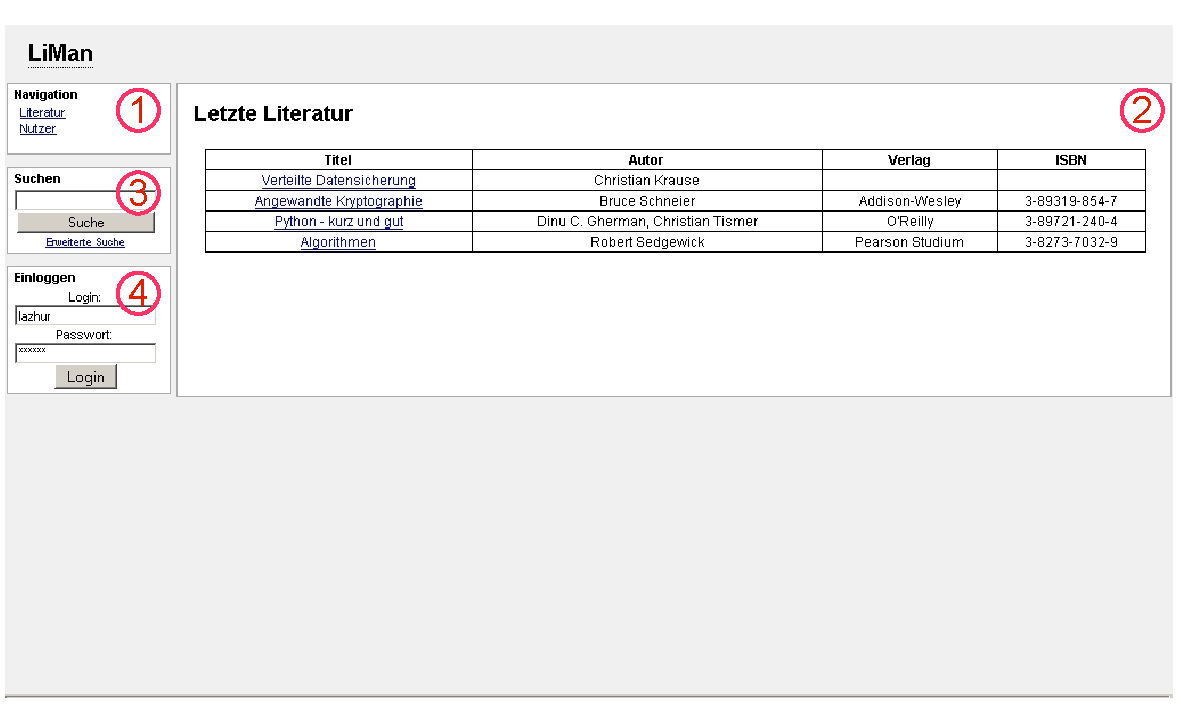
\includegraphics[scale=0.8]{screen1}\\
Die Hauptseite ist in vier Segmente aufgeteilt:\\
\begin{enumerate}
\item Navigation:\\
In dem Segment Navigation kann man nun zwischen zwei Men"upunkten w"ahlen:\\
Literatur und Nutzer\\
Auf diese beiden Punkte wird sp"ater genauer eingegangen.
\item Letzte Literatur:\\
Dieses Segment erm"oglicht einen "Uberblick der zuletzt get"atigten Literatureintr"age.
\item Suchen:\\
Die Suchfunktion erm"oglicht eine schnelle Recherche in den vorhandenen Literaturdaten. Die genauere Bedienung wird noch erl"autert.
\item Einloggen:\\
Hier kann sich jedes Mitglied mit seinem Login, also einem Namen und seinem Passwort bei dem Literaturmanager anmelden.\\
Sollte man keinen Login-Name und kein Passwort besitzen so muss man sich bei einem Administrator anmelden.\\
Auch wenn man sein Passwort vergessen hat, muss man einen Administrator kontaktieren.\\
\end{enumerate}
\subsection{Wie logge ich mich ein?}
Im Segment Einloggen auf der Hauptseite existieren zwei Editfelder, Login und Passwort.\\
Man gibt also in das obere Feld seinen Login-Namen und in das zweite Feld sein Passwort ein. Anschlie"send bet"atigt man den Button "Login" (1).\\
In der folgenden Abbildung ist der Abschnitt Einloggen einmal vergr"o"sert dargestellt.
Wir Loggen uns mit dem Namen 'Lazhur' und dem Passwort 'tescht' ein:\\
\begin{center}
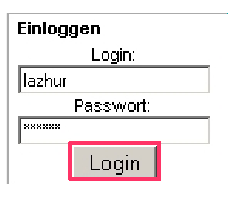
\includegraphics[scale=1.0]{login}\\
\end{center}
War die Anmeldung erfolgreich so erscheint folgende Anzeige und man ist als Mitglied eingeloggt:\\
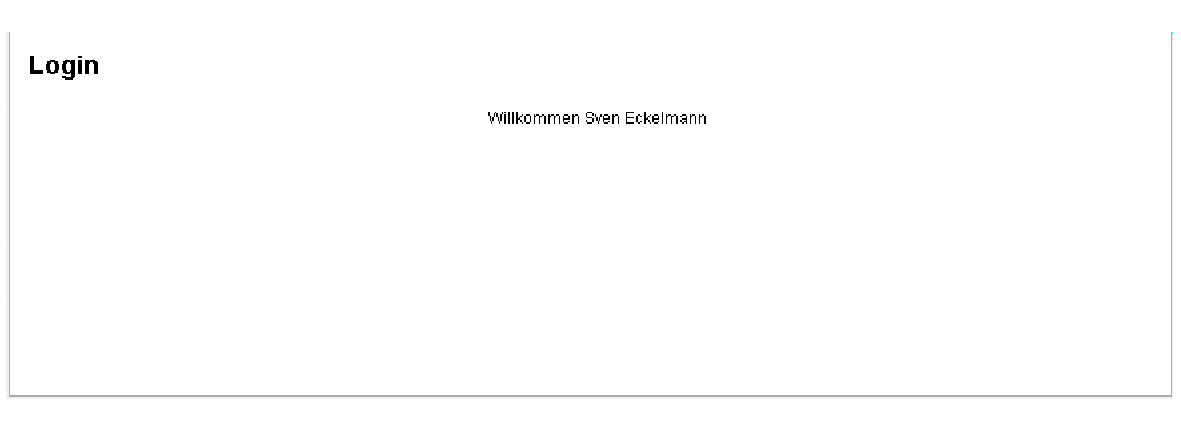
\includegraphics[scale=0.8]{login1}

\subsection{Wie finde ich eine Literatur?}
Um Informationen zu einem Literaturtitel zu erhalten bietet es sich an die Suchfunktion des Literaturmanagers zu nutzen. Hierzu kommen wir kurz auf das Bild des Hauptbildschirm weiter oben zur"uck:\\
Folgendes Bild verg"o"sert das Suchsegment (3):\\
\begin{center}
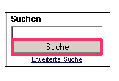
\includegraphics[scale=2.0]{suche}\\
\end{center}
Das Prinzip ist ganz einfach. Man gibt ein Stichwort zu einem Literaturtitel ein, z. B. ein Wort aus dem Titel oder den Namen des Autors, und dr"uckt den Suche-Button (1).\\
Gibt man z. B. den Begriff 'Python' ein so erscheinen alle Literaturtitel mit diesem Begriff. Die n"achste Abbildung zeigt einmal eine solche Trefferliste:\\
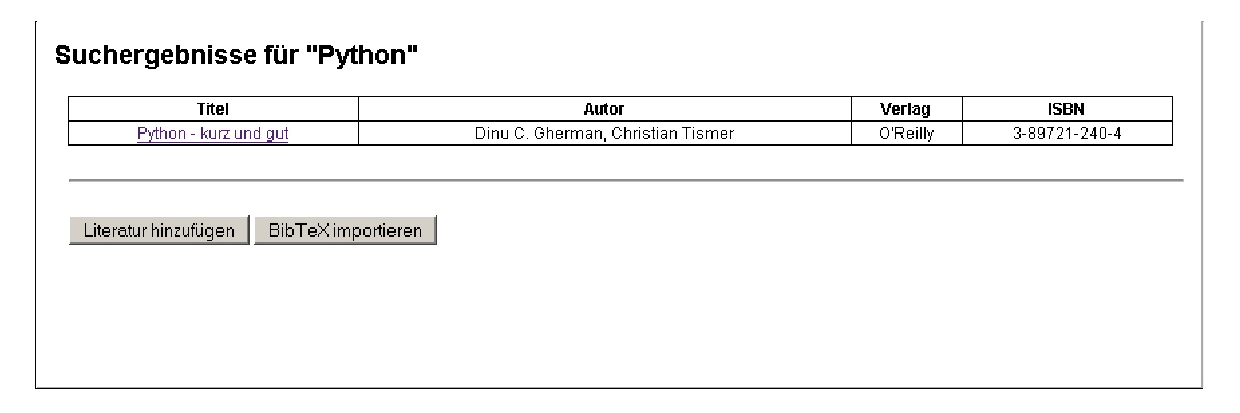
\includegraphics[scale=0.8]{treffer}\\
\subsection{Die erweiterte Suche}
Klickt in dem Suchsegments auf den Link 'Erweiterte Suche' so erscheint folgender Bildschirm:\\
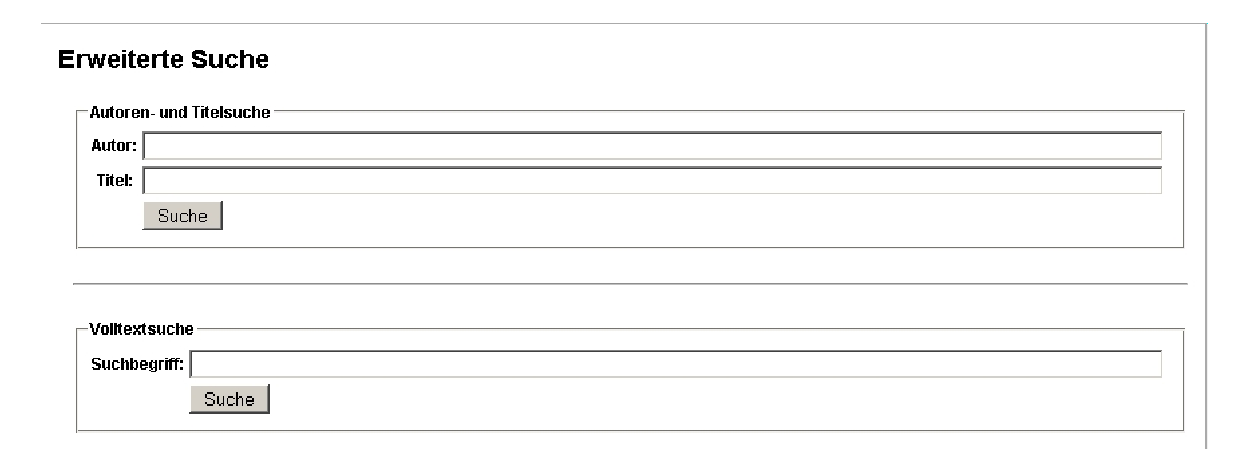
\includegraphics[scale=0.8]{ext_suche}\\
Die Suchfunktionen richten sich nunmehr auf spezielle Informationen eines Buches, was sich bei sehr gro"sen Datenbest"anden, die sich im Lauf der Zeit anreichern, in Form einer gr"o"seren "Ubersichtlichkeit der Suchtreffer auszahlen k"onnte.\\
Im Feld 'Titel' gibt man einfach einen Literatur-Titel , ein Wort aus dem Titel oder sogar nur eine kurze Zeichenkette wie 'Algo' ein.\\
Im Feld 'Autor' funktioniert es genau so, einfach einen Autor oder auch nur Teile seines Namens eingeben und den Button 'Suche' dr"ucken.\\
Die Volltextsuche sucht, "ahnlich wie die 'normale' Suche auf dem Hauptformular in allen Informationen eines Literaturtitels mit Ausnahme der Kommentare.

\subsection{Wie kann ich eine neue Literatur anlegen?}
Kommen wir nun vom Recherchieren zum bearbeiten und Pflegen der Literaturverwaltung.\\
Angenommen eine Literatur ist nicht in der Literaturverwaltung vorhanden und ein Mitglied m"ochte es darin aufnehmen.\\
Hierzu klicken wir zun"achst im Segment 'Navigation' auf den Punkt 'Literatur', daraufhin erscheint folgendes Fenster:\\
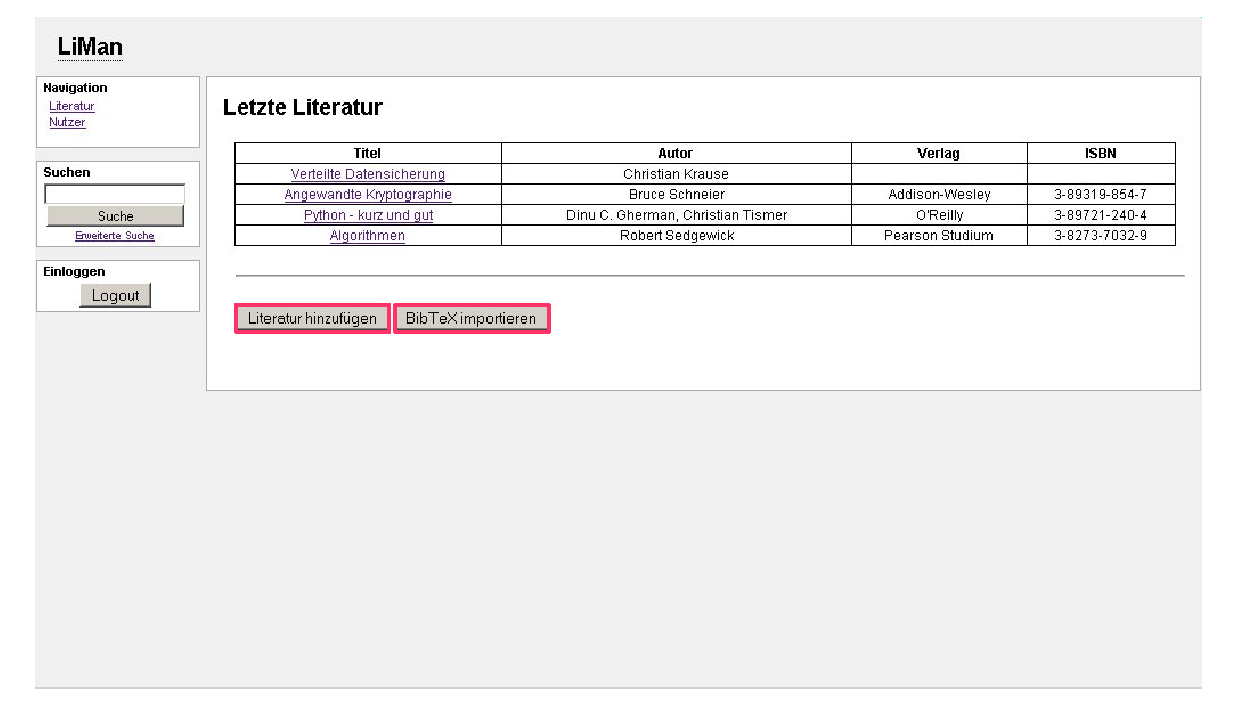
\includegraphics[scale=0.8]{lit_ins}\\
Dominiert wird das Segment von der Tabelle mit den Literatureintr"agen darunter befinden sich zwei Buttons, die nur dann erscheinen, wenn man sich als Mitglied angemeldet hat.\\
Der Button 'Literatur hinzuf"ugen' spricht wohl f"ur sich. Er erm"oglicht das hinzuf"ugen eines neuen Literaturtitels.\\
Der Button 'BibTex importieren' erm"oglicht es bereits vorgefertigte Literaturbeschreibungen im BibTex-Format zu importieren.\\
Klickt man nun auf den Button 'Literatur hinzuf"ugen' erscheint folgendes Formular:\\
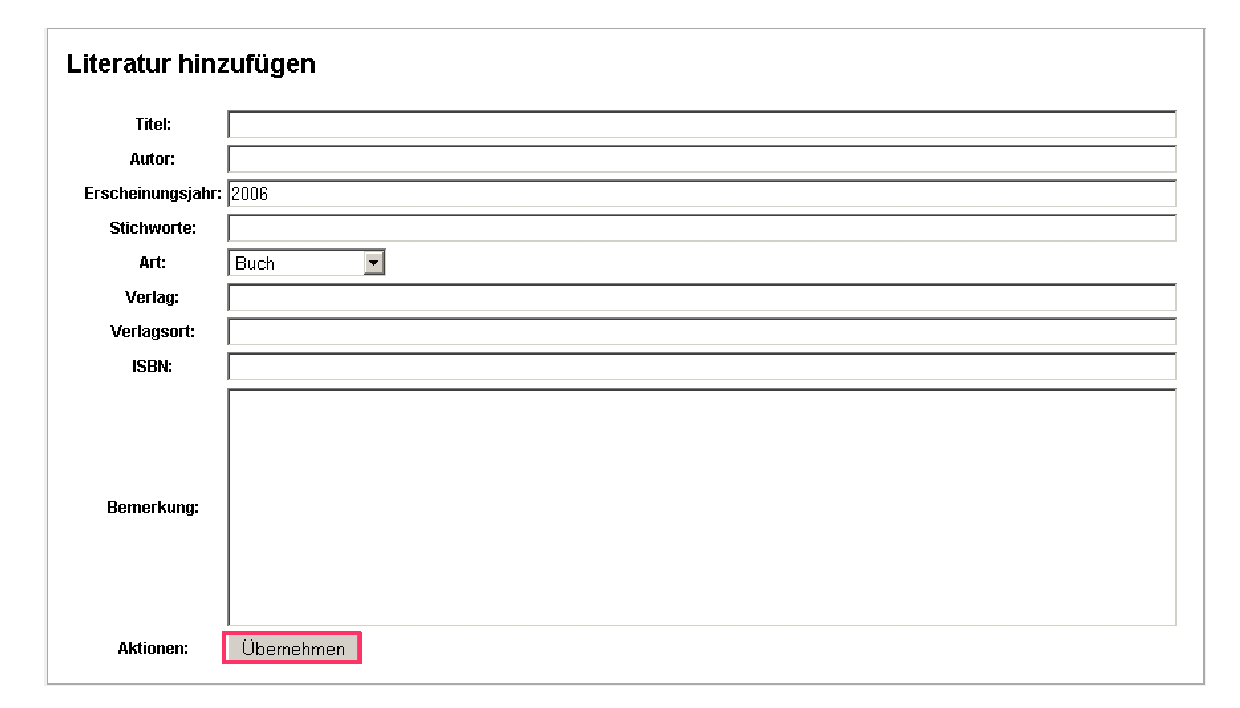
\includegraphics[scale=0.8]{lit_ins1}\\
Will man nun einen Eintrag in das Literaturverzeichnis machen, so muss man alle Felder ihrer Beschreibung gem"a"s auszuf"ullen und den Button '"Ubernehmen' dr"ucken.\\
F"ur einen von der Anwendung akzeptierten Eintrag sind die Felder 'Titel' und 'Autor' zwingend auszuf"ullen, sonst erscheint folgende Fehlermeldung:\\
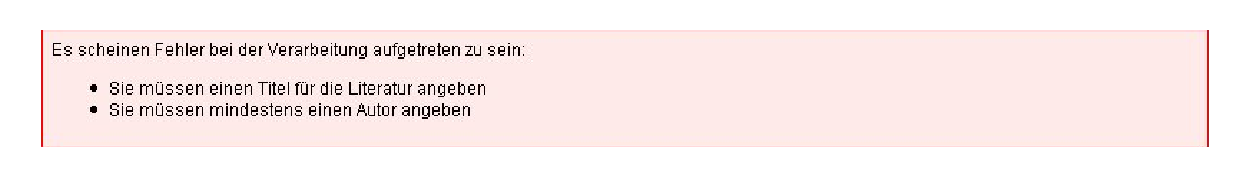
\includegraphics[scale=0.8]{err}

\subsection{Literatur mit BibTeX anlegen}
W"ahlt man statt dem Web-Formular zum Literatur-Import den Import via BibTeX, so sieht man sich folgendem Formular konfrontiert:\\
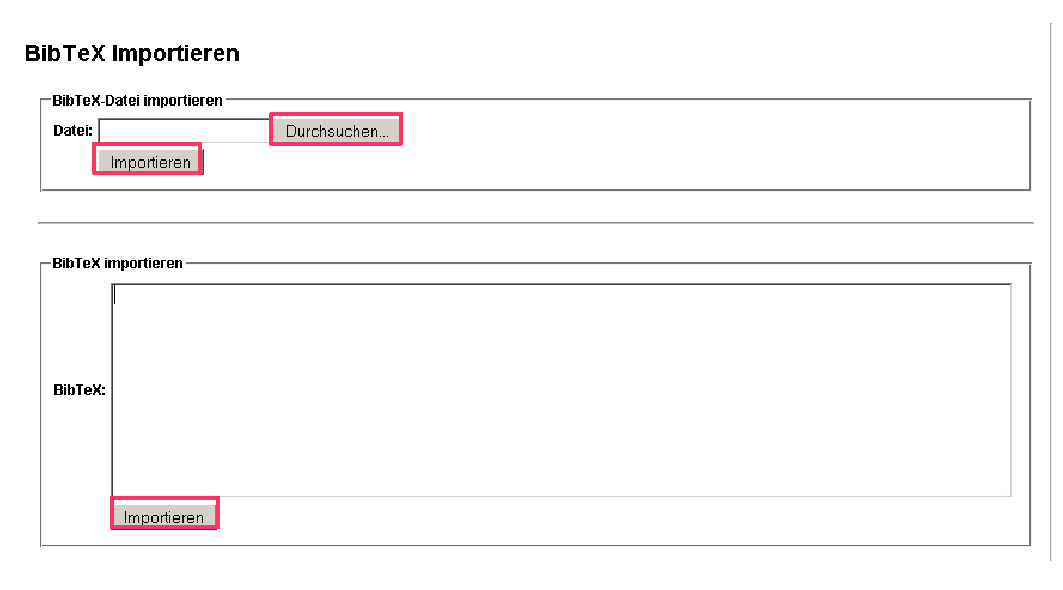
\includegraphics[scale=0.8]{bibtex}\\
Auch hier deuten zwei Segmente auf zwei M"oglichkeiten die BibTeX-Beschreibung zu importieren.\\
Die erste M"oglichkeit ist es, ein lokale BibTeX-Datei vom Computer des Mitglieds einzulesen. Hierzu klickt man auf 'Durchsuchen' und w"ahlt in dem lokalen Verzeichnisbaum die BibTeX-Datei aus und dr"uckt den "Offnen-Button. Folgendes Bild zeigt den "Offnen-Dialog indem man die Datei ausw"ahlen kann:\\
\begin{center}
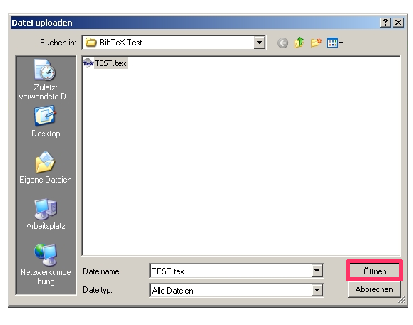
\includegraphics[scale=0.8]{import1}\\
\end{center}
Nachdem man die BibTeX-Datei ausgew"ahlt hat, dr"uckt man noch den Button 'Importieren' und ein neuer Literatureintrag wurde get"atigt.\\[0.4cm]
Die zweite M"oglichkeit ist die direkte Eingabe der BibTeX-Beschreibung in das Memo-Feld im zweiten, unteren Segment des Import-Formulars.\\
Folgendes Bild zeigt ein Beispiel:\\
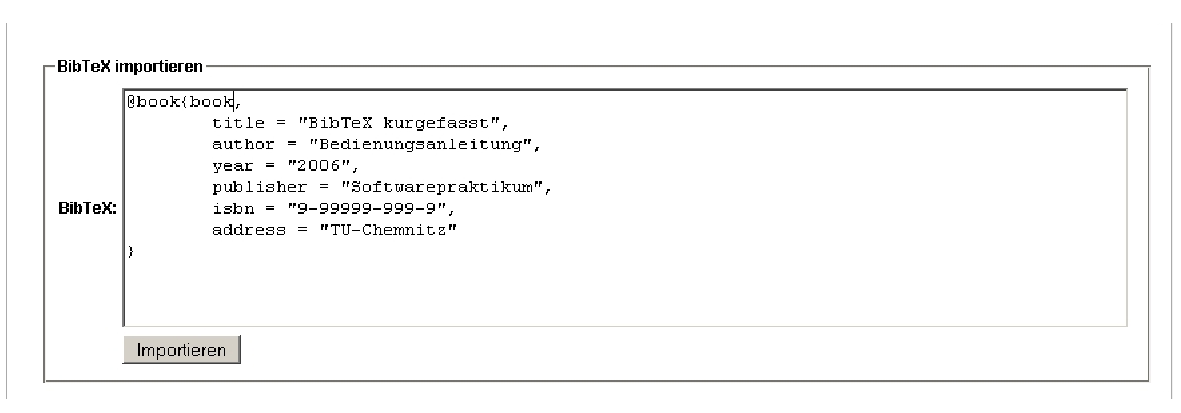
\includegraphics[scale=0.8]{import2}\\
Nach der Eingabe der Beschreibung muss man noch den Button 'Importieren' dr"ucken und ein neues Buch mit Titel 'BibTeX kurzgefasst' wurde in die Literaturverwaltung aufgenommen.\\
Der efolgreiche Import wird durch folgende Anzeige signalisiert:\\

\includegraphics[scale=0.8]{import_succ}

Beim Einfügen von BibTeX-Daten ist darauf zu achten, dass nur je ein Attribut auf einer Zeile steht. Bei mehr als einem Attribut kann nicht garantiert werden, dass eine korrekte Trennung der einzelnen Attribute durchgeführt wird. Außerdem sollte direkte Einbettung von LaTeX-Befehle vermieden werden. Sollte dies trotzdem einmal passieren, muss der Literatureintrag nachträglich bearbeitet werden.

\subsection{Wie bearbeite ich eine Literatur?}
M"ochte man einen Literatureintrag "andern, etwa weil man einen Fehler bei der Erstellung gemacht hat oder um eine Aktualisierung vorzunehmen, muss man sich zun"achst die Literaturtabelle anzeigen lassen, danach den zu "andernden Eintrag ausw"ahlen und den Button 'Bearbeiten' dr"ucken.\\
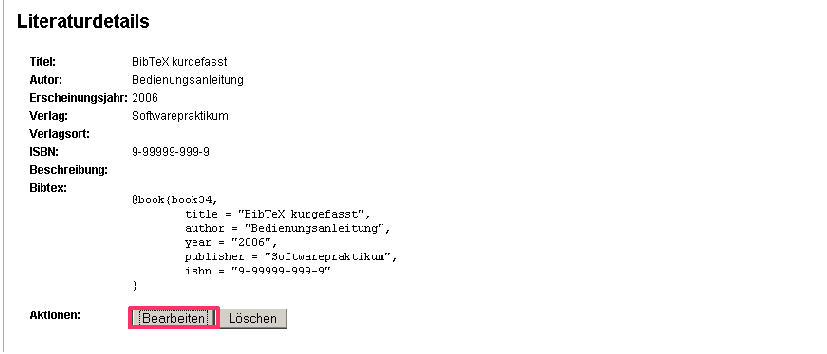
\includegraphics[scale=0.8]{bearb1}\\
Anschlie"send erscheint ein Formular "ahnlich dem Formular 'Literatur erstellen' nur stehen bereits Literatur-Information in den Feldern.
Im folgenden Bild wollen wir eine "Anderung an unserem erstellten Literatur-Titel 'BibTeX kurzgefasst' vornehmen, wir wollen die ISBN von 9-99999-999-9 in 0-00000-000-0 "andern und Verlag in SwP umbenennen:\\
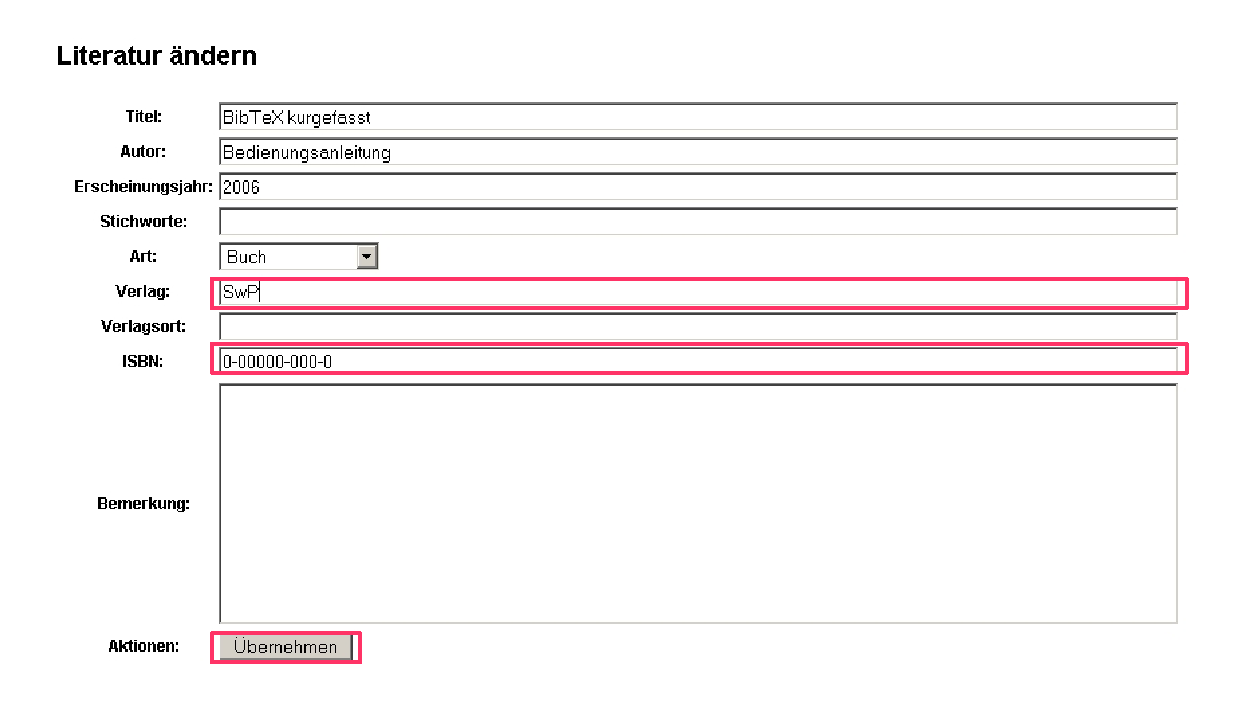
\includegraphics[scale=0.8]{bearb2}\\
Anschlie"send noch '"Ubernehmen' dr"ucken und unsere Literaturdaten wurden ge"andert. Best"atigt wird die "Anderung durch folgende Meldung:\\

\includegraphics[scale=0.8]{bearb3}

\subsection{Wie l"osche ich eine Literatur?}
Ist es n"otig einen Literatureintrag zu l"oschen, so w"ahlt man ihn wie auch beim 'Bearbeiten' in der Literaturliste aus, l"asst sich also die betreffenden Literaturdetails anzeigen, und bet"atigt den Button 'L"oschen':\\
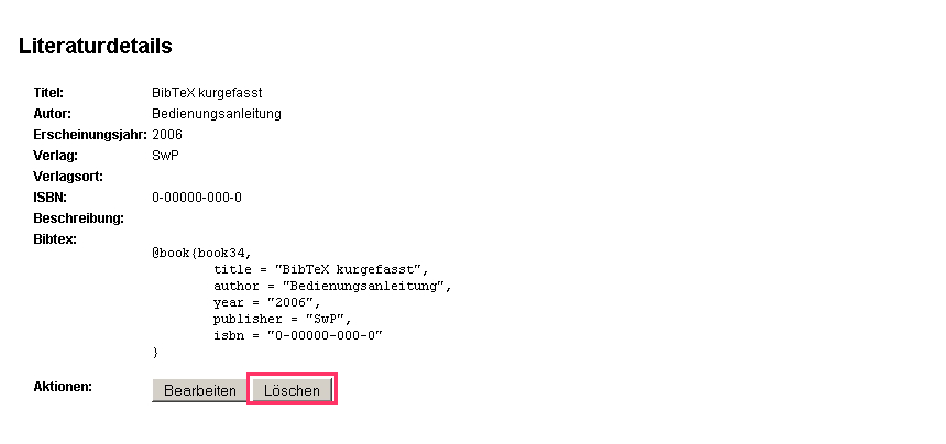
\includegraphics[scale=0.8]{del_lit}\\
Daraufhin erscheint die Aufforderung den L"oschvorgang zu best"atigen. Sollten man es sich anders "uberlegt haben, so bet"atigt man NICHT den Best"atigen-Button sondern verl"asst "uber das seitliche Men"u oder den Zurück-Knopf des Browsers den L"oschprozess.\\
Sollte man sich sicher sein, dass man den Eintrag l"oschen will, so klickt man auf den Button 'Best"atigen':\\

\includegraphics[scale=0.8]{sure}


\subsection{Wie kommentiere ich einen Literatureintrag?}
Oftmals ist ein kurzer Kommentar eines Lesers eines Buches oder einer Zeitschrift wesentlich aussagekr"aftiger als alle fachlichen Beschreibungen, die man findet.\\
M"ochte man nun einen solchen Kommentar zu einem Literatureintrag verfassen, etwa weil man das jeweilige Medium bereits gelesen oder zu Recherchen herangezogen hat muss man zun"achst, wie auch beim l"oschen und bearbeiten eines Eintrages, sich die Literaturdetails anzeigen lassen.\\
Bei niedriegeren Aufl"osungen, etwa 800x600 oder noch niedriger, k"onnte es n"otig sein mit der Laufleiste rechts von den Details in den unteren Bereich des Segments zu scrollen.\\
Dort findet man ein Textfeld worin man seinen Kommentar verfassen kann, anschlie"send best"atigt man ihn mit dem Button 'Kommentar versenden':\\
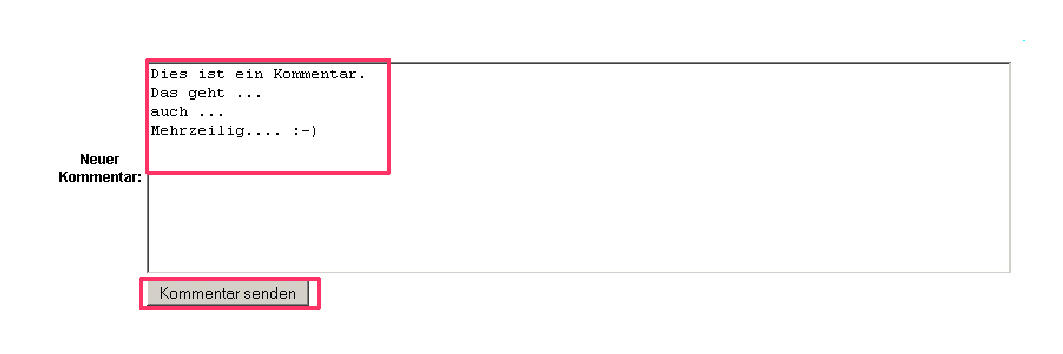
\includegraphics[scale=0.8]{comment1}\\
Auch hier erfolgt eine visuelle Best"atigung "uber die erfolgreiche Abgabe eines Kommentars:

\includegraphics[scale=0.8]{comment2}\\
Mit dem Button 'Zur"uck' gelangt man zu den Literaturdetails des gerade kommentierten Titels zur"uck.

\subsection{Wie "andere ich einen Kommentar?}
Will man einen seiner Kommentare zu einem Literaturtitel "andern, muss man den gew"unschten Titel in der Literaturliste ausw"ahlen um sich die Details anzeigen zu lassen.\\
Scrollt man nun zu den Kommentaren, so sieht man in dem Textfeld, welches bereits beim Erstellen eines Kommentars n"otig war, den Kommentar, den man zuvor abgegeben hatte.\\
M"ochte man den zuvor abgegeben Kommentar "andern, so formatiert man ihn jediglich in diesem Textfeld und bet"atigt erneut 'Kommentar senden'.\\
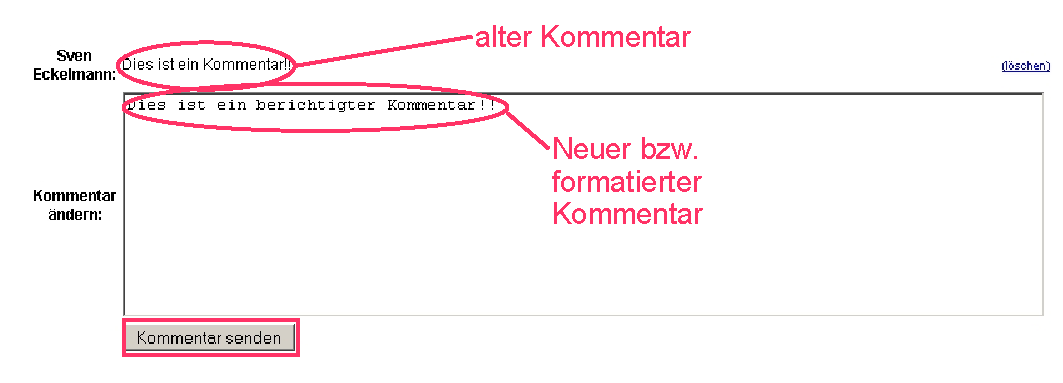
\includegraphics[scale=0.8]{comment3}\\
Es erscheint eine Best"atigung "ahnlich der, die beim Verfassen eines Kommentares erscheint.\\

\subsection{Wie l"osche ich einen Kommentar?}
Ist es n"otig einen seiner verfassten Kommentare zu l"oschen, muss man sich wieder die Literaturdetails des Literaturtitels anzeigen lassen, worin der zu l"oschende Kommentare steht.\\
Sucht man den Kommentar, hinter dem ein Link mit der Aufschrift l"oschen steht und bet"atigt diesen. Die folgende Abbildung soll dies verdeutlichen:\\
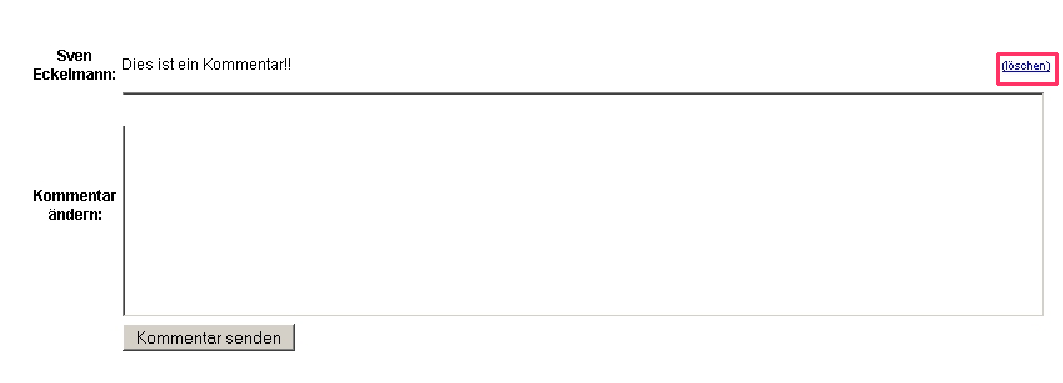
\includegraphics[scale=0.8]{comment4}\\
Bet"atigt man diesen Link, so erscheint als n"achstes eine L"oschbest"atigung. Hier gilt Selbiges wie auch beim L"oschen von Literatur, will man den Vorgang abbrechen geht man einfach "uber die Men"uleiste am linken Browser-Rand in ein anderes Men"u. Ist man sich sicher, dass man den Kommentar l"oschen will so bet"atigt man den Button.\\

\includegraphics[scale=0.8]{comment5}\\
Nachdem man den Best"atigen-Button benutzt hat, erscheint eine L"oschbest"atigung.

\subsection{Wie kann ich meine Mitgliedsdaten "andern?}
Grunds"atzlich gilt, dass jedes Mitglied die eigenen Mitgliedsdaten "andern darf.\\ Man benutzt einfach im Navigationssegment den Men"upunkt 'Nutzer'. Tut man dies, so erscheint folgende "Ubersicht:\\
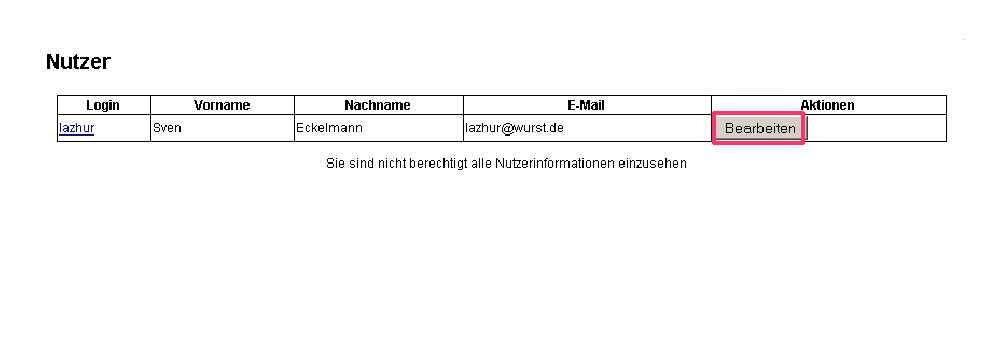
\includegraphics[scale=0.8]{nutzer1}\\
Wie man leicht erkennen kann, hat man als Mitglied jediglich das Recht die eigenen Nutzerdaten zu sehen und zu "andern.\\
Bet"atigt man nun den Button 'Bearbeiten' so erh"alt man Zugang zu den eigenen Mitgliedsinformationen.\\
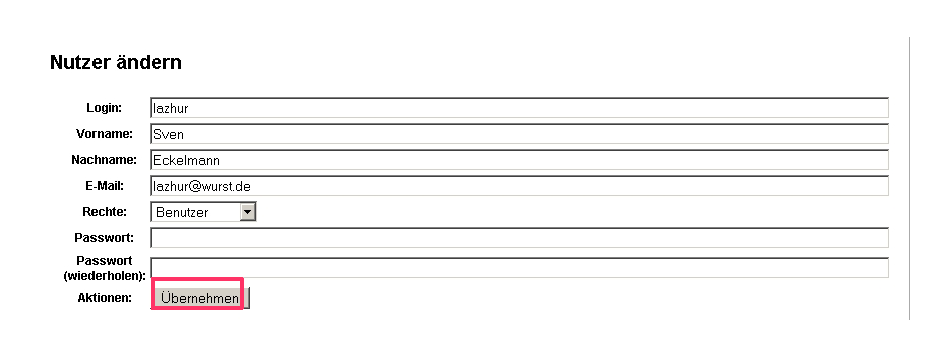
\includegraphics[scale=0.8]{nutzer2}\\
M"ochte man beispielsweise seine E-Mail-Adresse "andern, l"oscht man einfach die alte Adresse raus und schreibt seine neue hinein. Danach best"atigt man mit dem Button '"Ubernehmen'.\\
Jedes Mitglied kann alle eigenen Daten, bis auf die 'Rechte', auf diese Wiese "andern. Allerdings ist das "Andern der Rechte einzig und allein Administratoren "uberlassen.\\
Danach erscheint eine Best"atigung "uber die "Anderung der Nutzerdaten.\\

\subsection{Ein"uhrung in die Nutzerverwaltung "uber die grafische Oberfl"ache der Literaturverwaltung}
Grunds"atzlich gilt, dass man "Anderungen in den Nutzerdaten der Mitglieder ausschlie"slich als Administrator durchf"uhren darf.\\
Um in die Nutzerverwaltung zu gelangen, befolgt man zun"achst die selben Anweisungen, wie sie im Punkt 3.4.4 'Wie logge ich mich ein?' aufgef"uhrt sind.\\
Hat man sich eingeloggt geht man im Segment Navigation (siehe 3.4.2 'Die Hauptseite') in das Untermen"u 'Nutzer'.\\
Im Gegensatz zur Mitgliedsoberfl"ache, sind nun alle Mitglieder aufgelistet.

\subsection{Wie lege ich einen Nutzer an?}
Hierzu klicken wir zun"achst im Segment 'Navigation' auf den Punkt 'Nutzer', daraufhin erscheint das Fenster Nutzer:\\
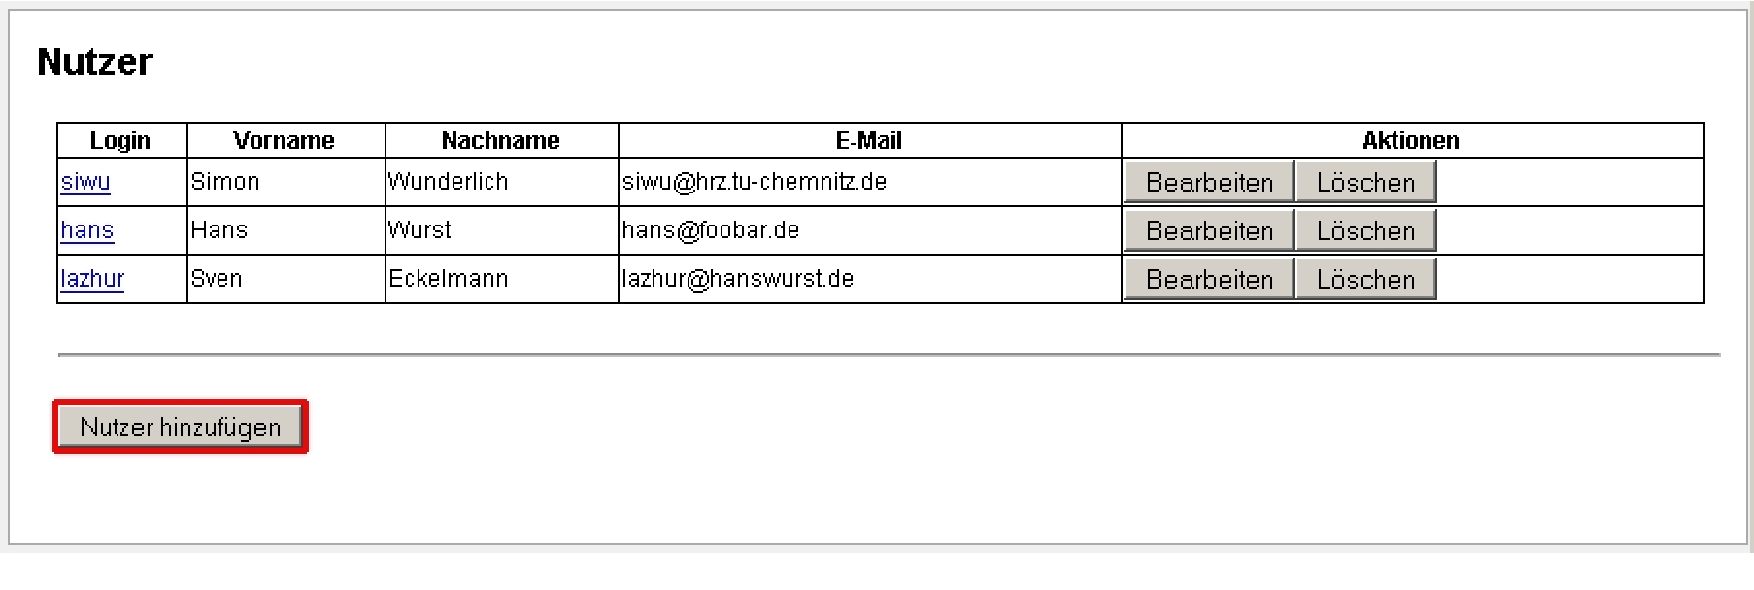
\includegraphics[scale=0.5]{nutzeranl}\\
Wenn man hier auf den Button 'Nutzer hinzuf"ugen' klickt, kommt man zu folgendem Formular:\\

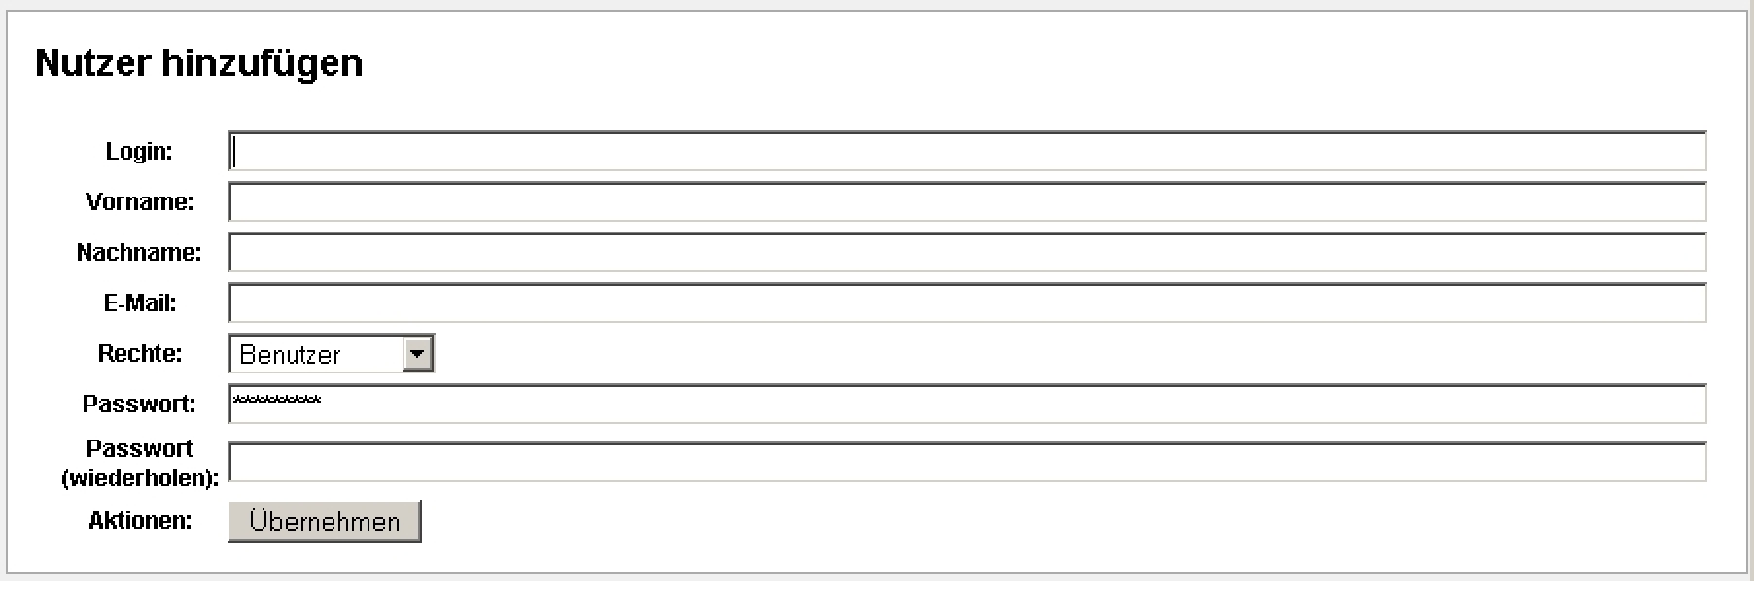
\includegraphics[scale=0.5]{nutzeranl2}\\
Will man nun einen Nutzer hinzuf"ugen, so muss man alle Felder ihrer Beschreibung gem"a"s auszuf"ullen und den Button '"Ubernehmen' 
dr"ucken. F"ur einen von der Anwendung akzeptierten Eintrag m"ussen alle Felder richtig ausgef"ullt sein, sonst k"onnen folgende Fehlermeldungen 
erscheinen: (Zur Demonstration sind alle Felder leer, um alle Fehlermeldungen anzuzeigen)\\
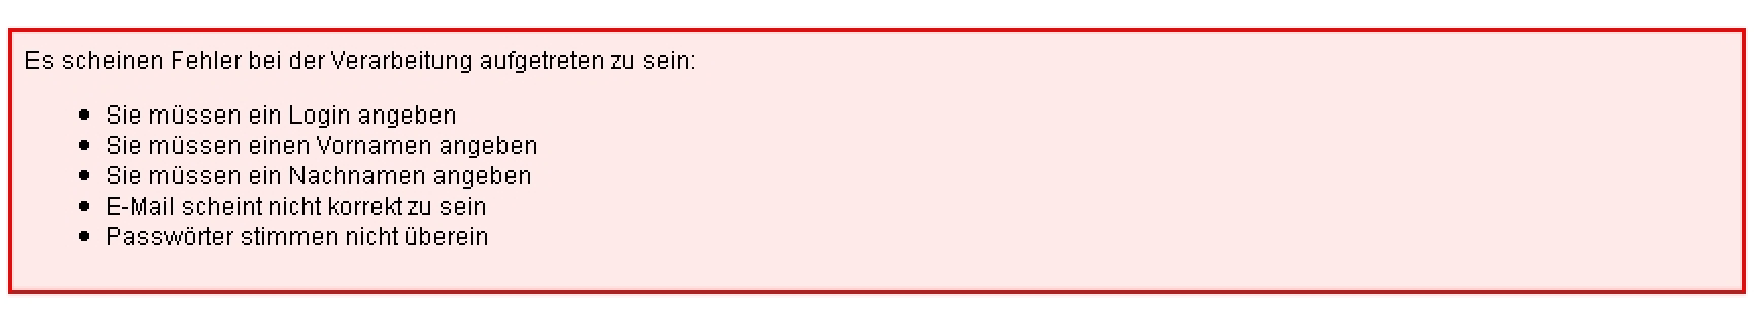
\includegraphics[scale=0.5]{nutzeranl3}\\
Wenn man die Felder korrekt ausgef"ullt hat und der Nutzer angelegt werden konnte kommt folgende Meldung:\\
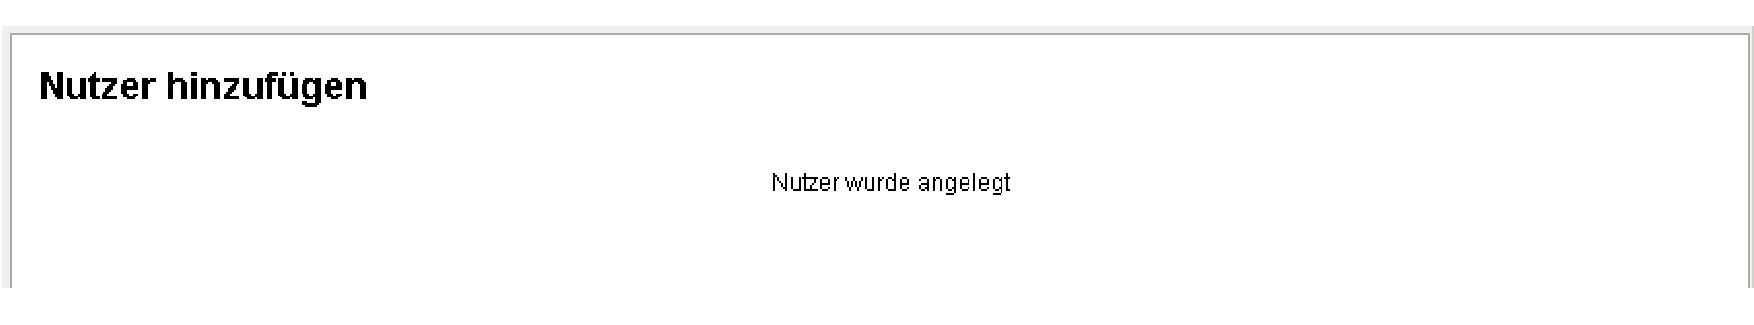
\includegraphics[scale=0.5]{nutzeranl4}

\subsection{Wie bearbeite ich einen Nutzer?}
Um einen bereits angelegten Nutzer zu bearbeiten, klicken wir zun"achst im Segment 'Navigation' auf den Punkt 'Nutzer', daraufhin erscheint das Fenster 
Nutzer:\\
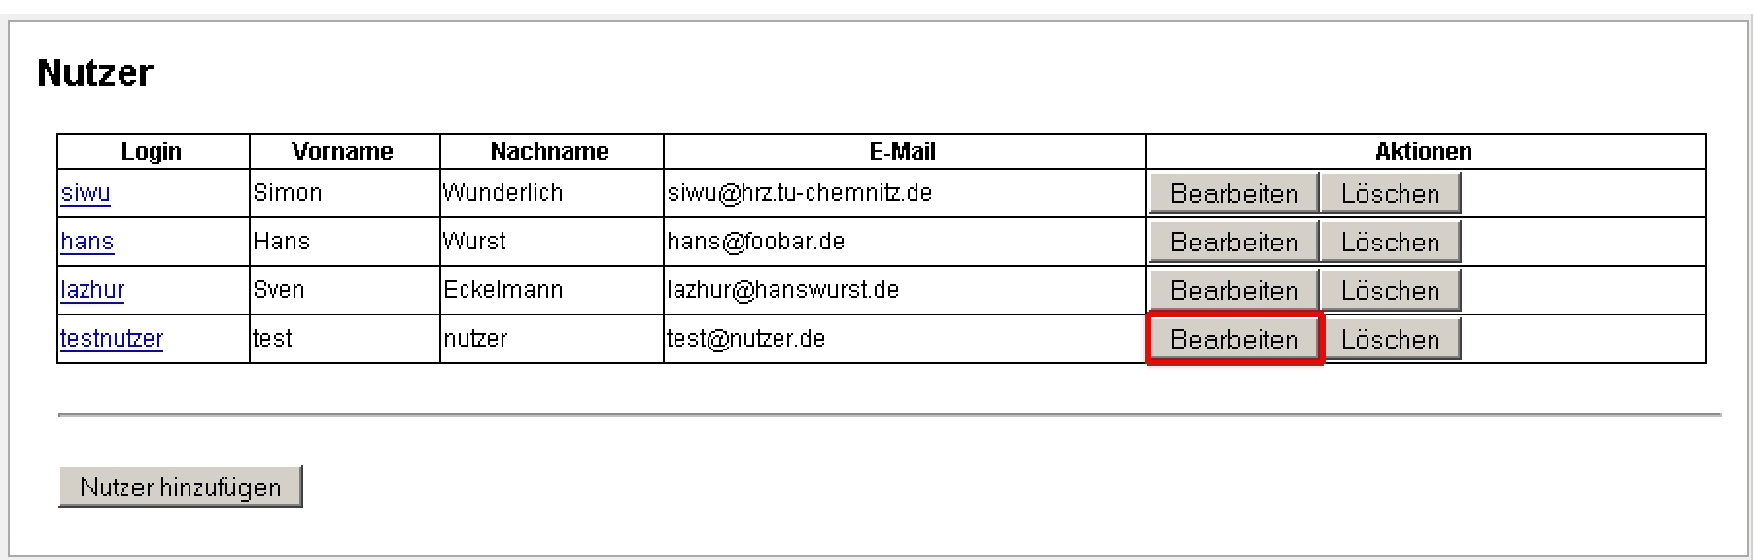
\includegraphics[scale=0.5]{nutzerbea}\\
Wenn man zum Beispiel den Nutzer 'testnutzer' bearbeiten will, so klickt man auf den Bearbeitungsbutton in der jeweiligen Zeile.
Das schon aus dem Abschnitt 'Wie lege ich einen Nutzer an?' bekannte Formular erscheint und man kann s"amtliche Daten "andern.\\
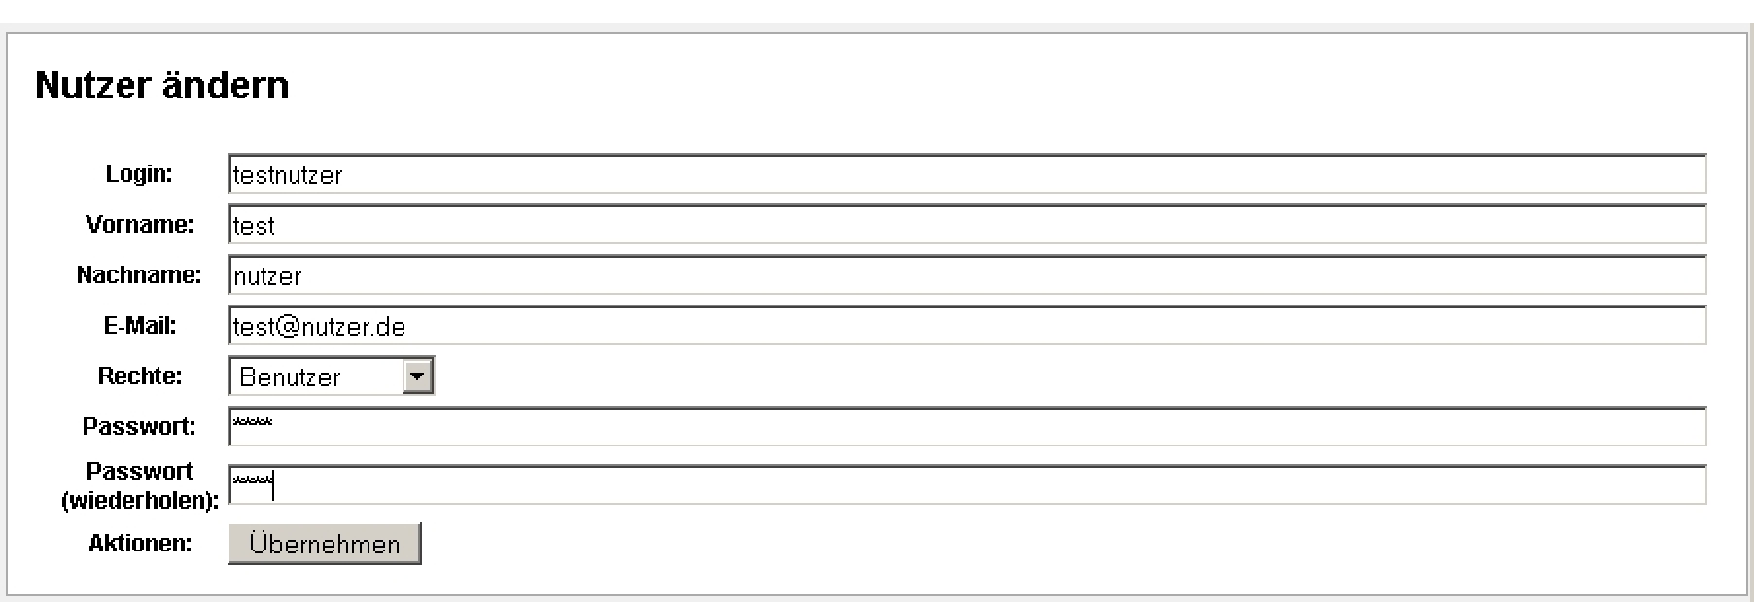
\includegraphics[scale=0.5]{nutzerbea2}\\
Wenn der Nutzer erfolgreich bearbeitet wurde, erscheint folgende Nachricht:\\
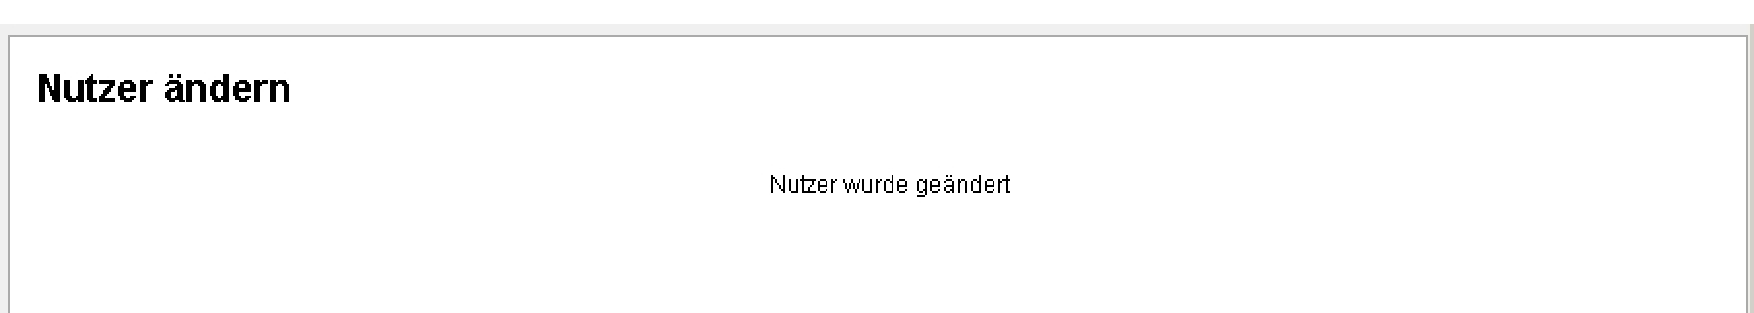
\includegraphics[scale=0.5]{nutzerbea3}

\subsection{Wie l"osche ich einen Nutzer?}  
Um einen Nutzer zu l"oschen, klicken wir zun"achst im Segment 'Navigation' auf den Punkt 'Nutzer', daraufhin erscheint das Fenster 
Nutzer:\\
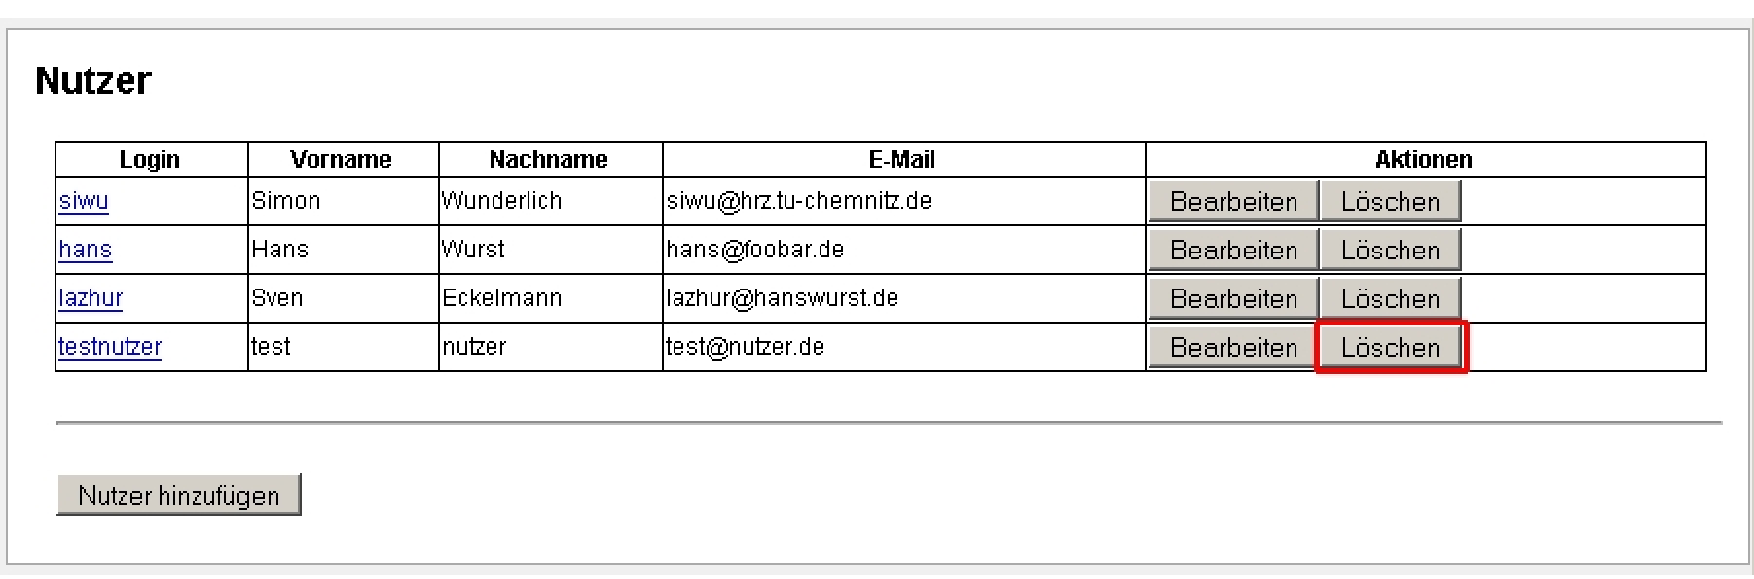
\includegraphics[scale=0.5]{nutzerloe}\\
Wenn man zum Beispiel den Nutzer 'testnutzer' l"oschen will, so klickt man auf den L"oschbutton in der jeweiligen Zeile.
Es erscheint eine Frage, ob sie den Nutzer wirklich entfernen wollen:\\
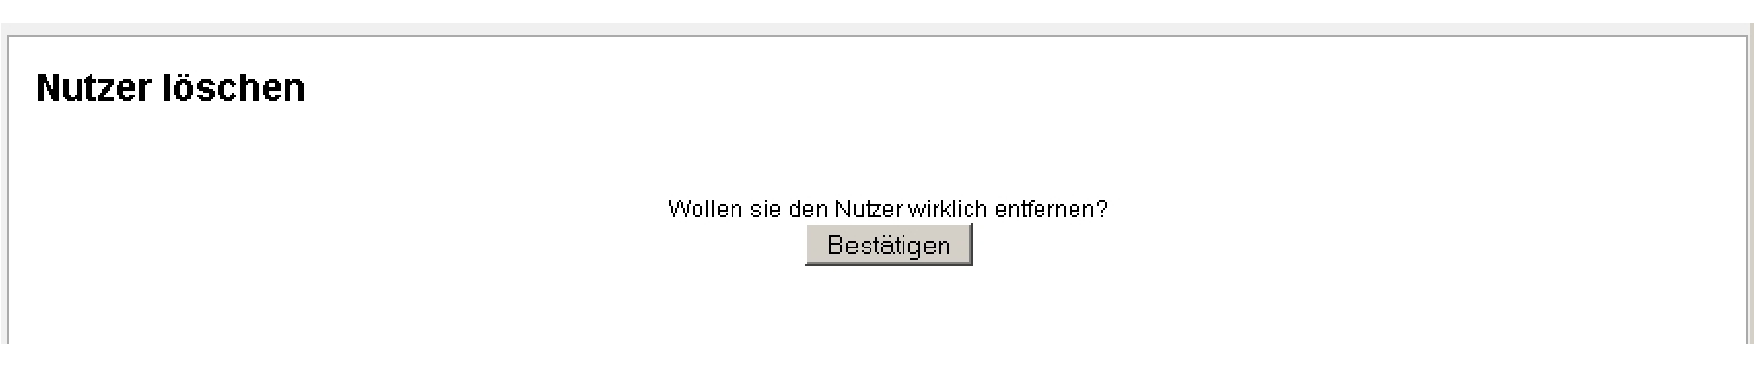
\includegraphics[scale=0.5]{nutzerloe2}\\
Wenn der Nutzer entfernt wurde, erscheint folgende Nachricht:\\
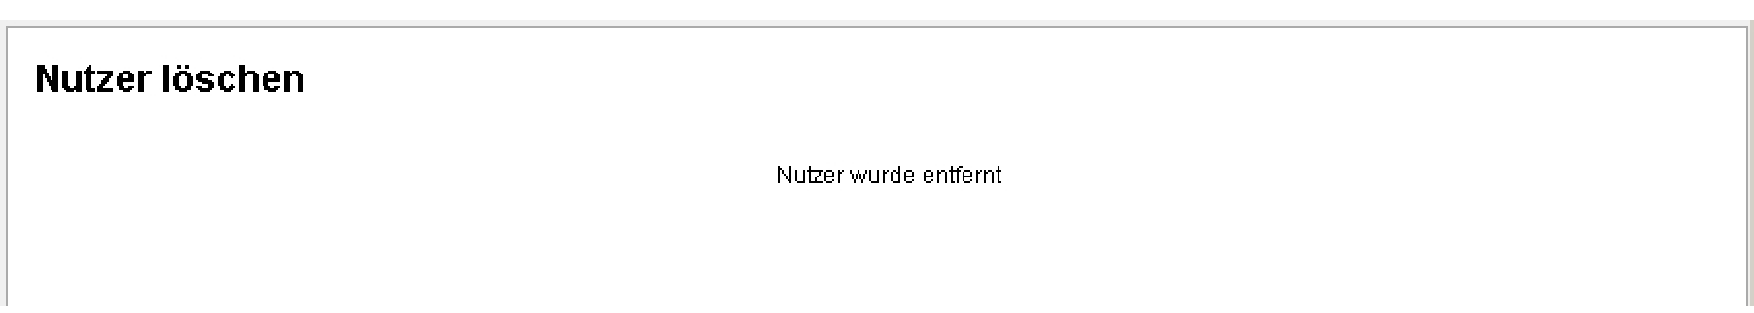
\includegraphics[scale=0.5]{nutzerloe3}

\section{Helpsystem}
Die Nachrichten beim Anlegen, Editieren und L"oschen von Datenbest"anden sind als Hilfestellung v"ollig ausreichend.\\
Ausserdem sind die Fehlermeldungen, die bei unzureichender Eingabe erscheinen, aussagekr"aftig genug.
